\subsection{Quicksort}
The Quicksort program is an implementation of tail recursive quicksort algorithm. It takes as input an array of integers and sorts the array. The base case for recursion is an array of size 1. When an array is size 1 is received , the function does nothing and returns. In the approximate version of the function the base case is changed from size 1 to knob. The approximate version does nothing whenever an array of size less than or equal to knob is received. This effectively limits the recursion process. Like bubblesort the accuracy measure is based on the number of inversions that are successfully removed from the array. In order to check the accuracy, the same set of 1000 arrays of 1000 elements are used that was used to test bubble sort.

For quicksort, PLATIN was not able to compile the modified version of the benchmark for WCET analysis. Therefore the WCET estimate for this one is measurement based. For quicksort, the worst possible case is that it always picks a bad pivot. The input and code is modified to trigger this case and WCET is measured through simulation. Table \ref{quicksortT} shows the results. From the table we can answer our questions as follows:

\begin{table}[]
  \centering
  \caption{Quicksort Results}
  \label{quicksortT}
  \begin{tabular}{|l|l|l|l|}
    \hline
    \textbf{Recursion Limit} & \textbf{Accuracy}  & \textbf{Standard Dev.}  & \textbf{WCET}           \\ \hline
5\% &  99.81\% &0.01\% &99.98\%   \\ \hline
10\% &  99.50\% &0.03\% &99.96\%   \\ \hline
15\% &  99.17\% &0.04\% &99.93\%   \\ \hline
20\% &  98.85\% &0.07\% &99.90\%   \\ \hline
25\% &  98.51\% &0.08\% &99.87\%   \\ \hline
30\% &  98.19\% &0.11\% &99.83\%   \\ \hline
35\% &  97.86\% &0.13\% &99.82\%   \\ \hline
40\% &  97.53\% &0.17\% &99.77\%   \\ \hline
45\% &  97.19\% &0.19\% &99.72\%   \\ \hline
50\% &  96.86\% &0.22\% &99.66\%   \\ \hline
  \end{tabular}
\end{table}


\begin{figure}
  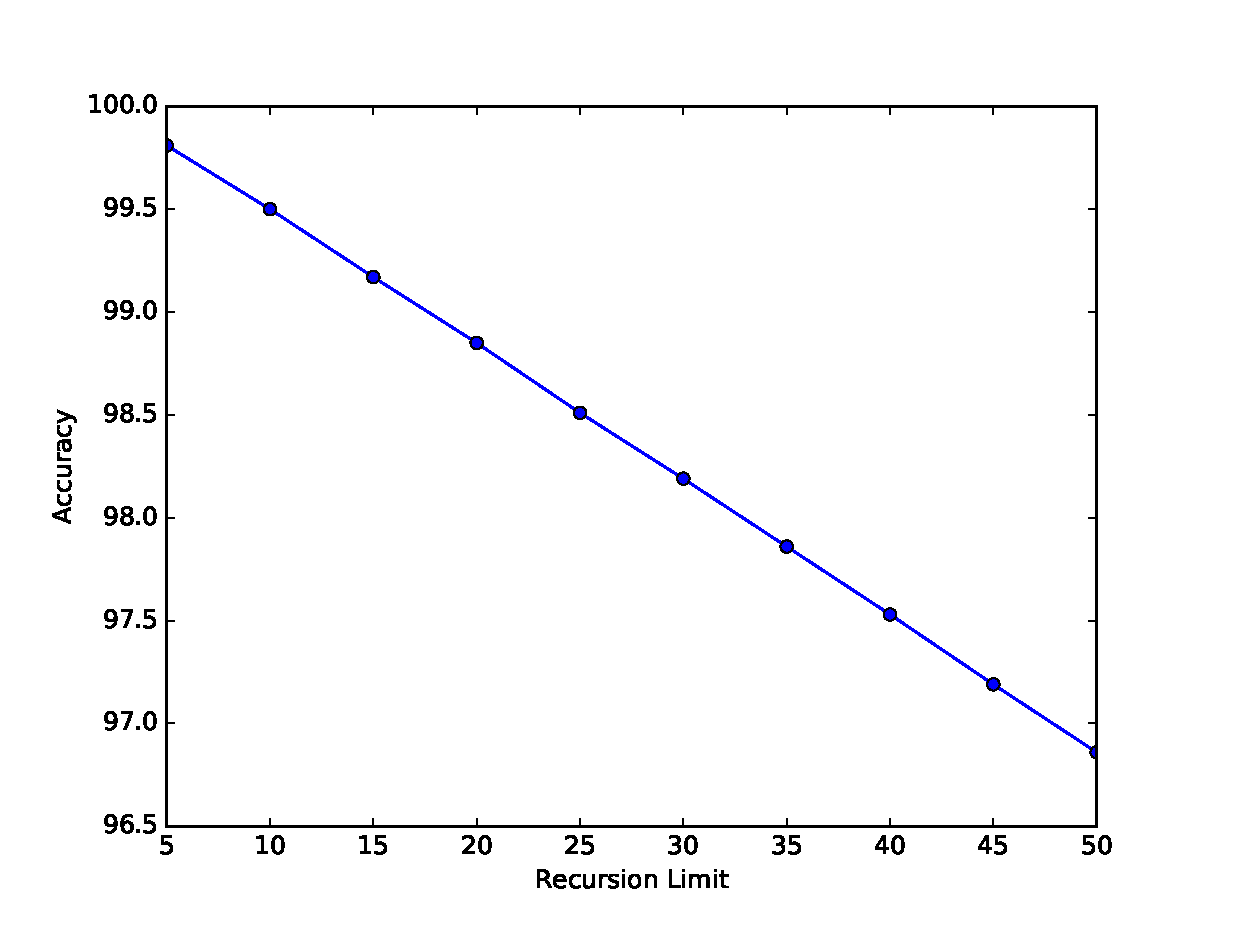
\includegraphics[width=0.95\linewidth]{Results/quicksort1.eps}
  \caption{Accuracy vs Recursion Limit}
  \label{quicksort1}
\end{figure}


\begin{enumerate}
\item The accuracy decreases linearly with recursion limit. This can be seen clearly from figure \ref{quicksort1}.
\item WCET decreases very slowly as recursion limit changes. This is because this recursion base case is being triggered only once when the quicksort is at its worst.
\item The approximation seems pointless since there is a 3\% accuracy loss for just 0.3\% decrease in WCET.
\end{enumerate}

\begin{table}[]
  \centering
  \caption{Quicksort Average Results}
  \label{quicksortT2}
  \begin{tabular}{|l|l|l|l|}
    \hline
    \textbf{Recursion Limit} & \textbf{Accuracy}  & \textbf{Standard Dev.}  & \textbf{Average Case Time}           \\ \hline
5\% &  99.81\% &0.01\% &80.96\%   \\ \hline
10\% &  99.50\% &0.03\% &72.27\%   \\ \hline
15\% &  99.17\% &0.04\% &67.59\%   \\ \hline
20\% &  98.85\% &0.07\% &64.16\%   \\ \hline
25\% &  98.51\% &0.08\% &61.28\%   \\ \hline
30\% &  98.19\% &0.11\% &58.75\%   \\ \hline
35\% &  97.86\% &0.13\% &56.92\%   \\ \hline
40\% &  97.53\% &0.17\% &55.77\%   \\ \hline
45\% &  97.19\% &0.19\% &53.74\%   \\ \hline
50\% &  96.86\% &0.22\% &51.28\%   \\ \hline
  \end{tabular}
\end{table}


\begin{figure}
  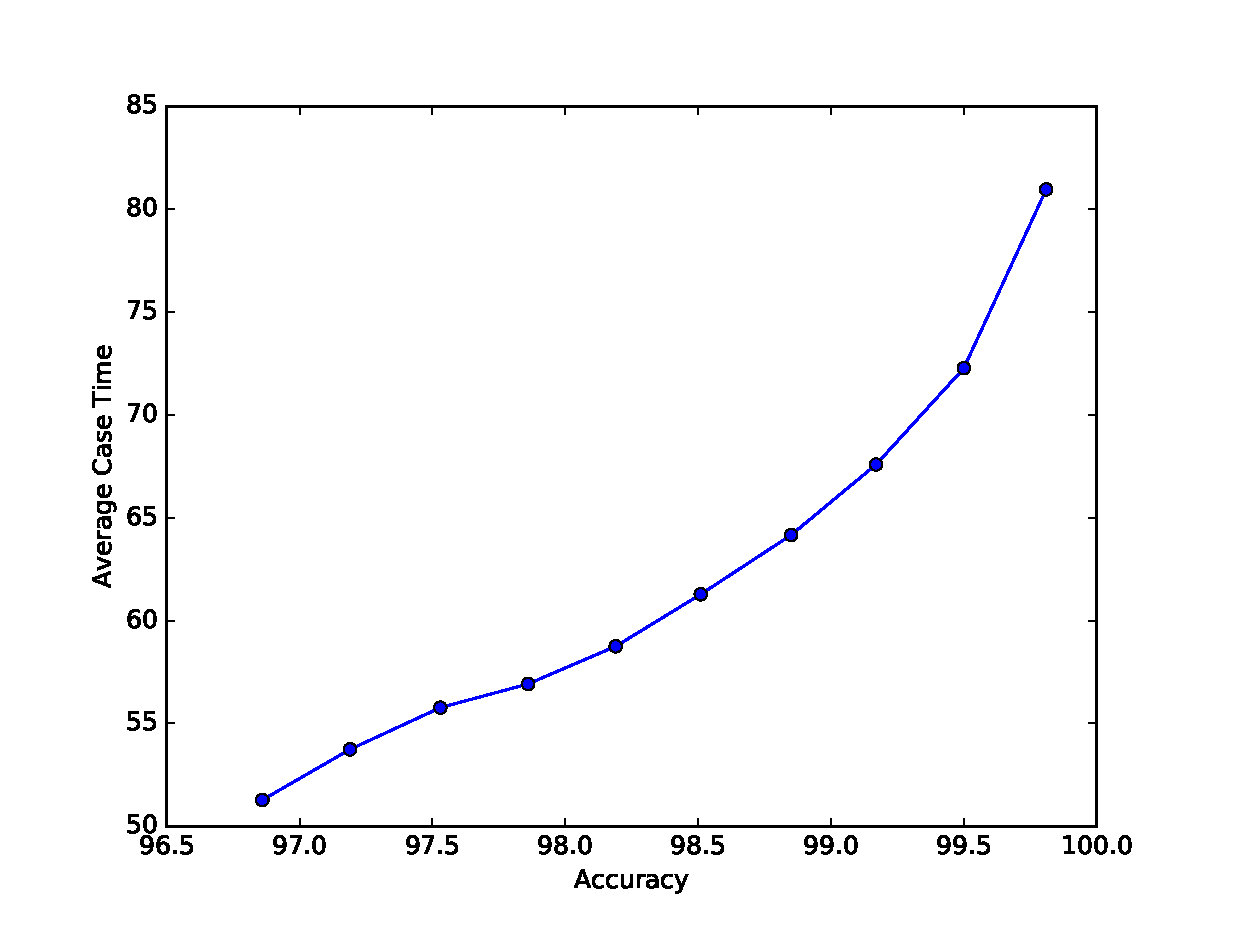
\includegraphics[width=0.95\linewidth]{Results/quicksort23.eps}
  \caption{Average Case Time vs Accuracy}
  \label{quicksort1}
\end{figure}

However the quicksort worst case is extremely improbable. In general, for a randomized algorithm like quicksort, the average case running time is of more interest. Table \ref{quicksortT2} shows the data for average case when random pivot is picked. Figure \ref{quicksort23} shows that the Average Case running time decreases quite sharply for a modest decrease in accuracy which make the approximation feasible for Average case.



%% \begin{figure}
%%   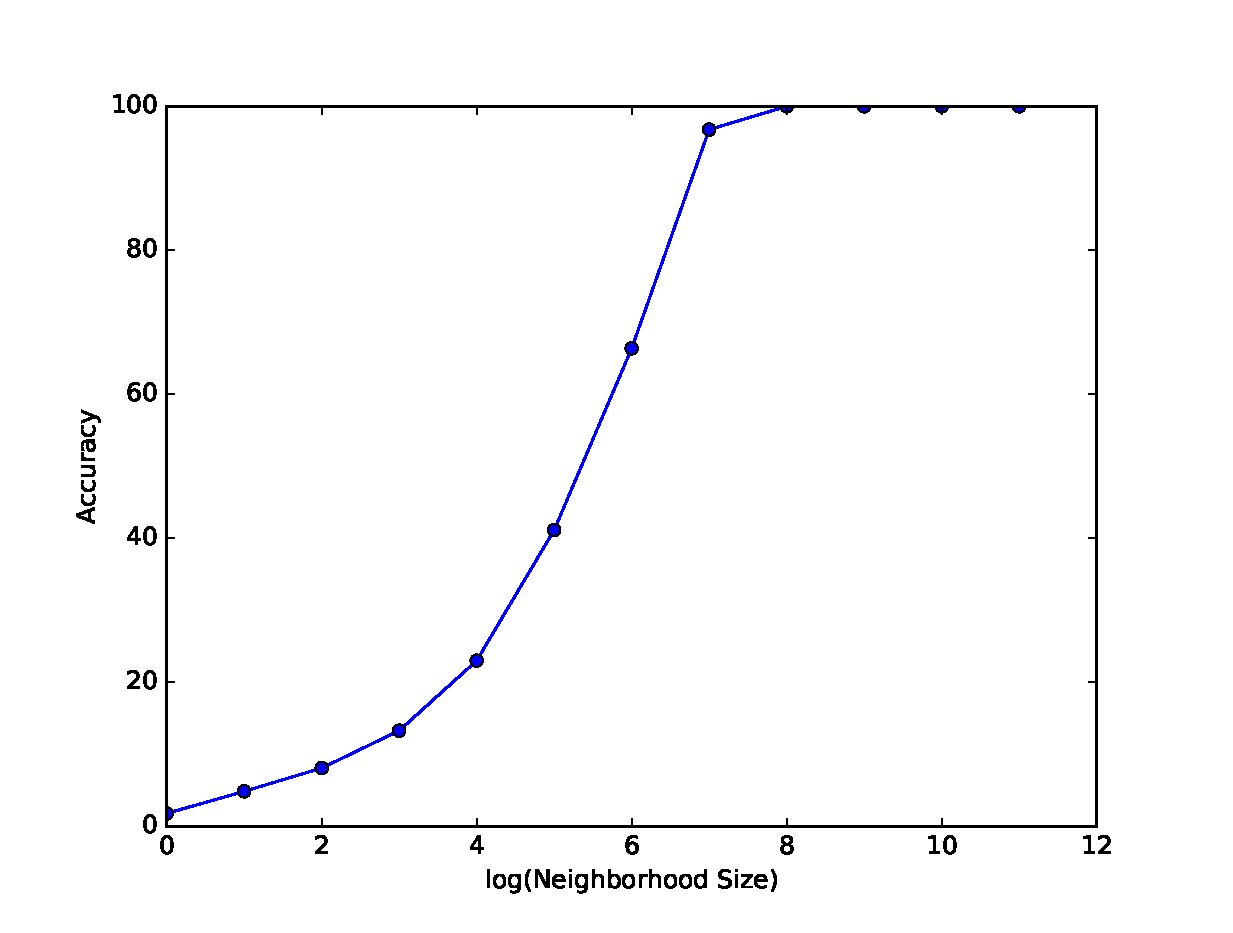
\includegraphics[width=0.95\linewidth]{Results/binarysearch1.eps}
%%   \caption{WCET vs Skipped Iterations)}
%%   \label{binarysearch2}
%% \end{figure}

